\lab{Algorithms}{Gibbs Sampling}{Gibbs Sampling}
\objective{Understand the basic principles of implementing a Gibbs sampler.}

Gibbs sampling is another Bayesian method in which we construct a Markov chain by which to sample from a desired joint posterior distribution 
\begin{equation*}
\mathbb{P}(x_{1},\cdots,x_{n} | \mathbf{y})
\end{equation*}
Often it is difficult to sample from this joint distribution, while it may be easy to sample from 
\begin{equation*}
\mathbb{P}(x_{i} | \mathbf{x}_{-i}, \mathbf{y})
\end{equation*}
where $\mathbf{x}_{-i} = x_{1},\cdots,x_{i-1},x_{i+1},\cdots,x_{n}.$

A Gibbs sampler proceeds as follows after a random initialization of all $x_{i}$:
\begin{enumerate}
	\item Pick a random index $1 \leq i \leq n$.
	\item Draw $x \sim \mathbf{P}(x_{i} | \mathbf{x}_{-i}, \mathbf{y})$.
	\item Fix $x_{i} = x$.
	\item Repeat.
\end{enumerate}

This creates an irreducible, non-null recurrent, aperiodic Markov chain over the state space consisting of all possible $\mathbf{x}$. The unique invariant distribution for the chain is the desired joint posterior distribution 
\begin{equation*}
\mathbb{P}(x_{1},\cdots,x_{n} | \mathbf{y})
\end{equation*}
Thus, after a burn in period, our samples $\mathbf{x}$ are effectively samples from the desired distribution.

One simplification is made in practice: the index $i$ is not drawn randomly, but rather simply incremented from $1$ to $n$. Thus the Gibbs sampler is as follows:
\begin{enumerate}
	\item Randomly initialize $\mathbf{x}$.
	\item For $1 \leq i \leq n$
	\begin{enumerate}
		\item Draw $x \sim \mathbb{P}(x_{i} | \mathbf{x}_{-i}, \mathbf{y})$.
		\item Fix $x_{i} = x$.
	\end{enumerate}
	\item Repeat (b).
\end{enumerate}

Each iteration of step (b) is a \emph{sweep} of the Gibbs sampler, and the value of $\mathbf{x}$ after a sweep is a sample.

Let us return to the case where we have exam scores from a calculus exam in the file \texttt{examscores.csv}. We believe that these exams should be normally distributed with mean $\mu$ and variance $\sigma^{2}$. We place priors on each parameter:
\begin{align*}
\mu & \sim N(\mu_{0}, \sigma_{0}^{2}) \\
\sigma^{2} & \sim IG(\alpha, \beta)
\end{align*}
Letting $\mathbf{y}$ be the exam scores, we would like to sample from the posterior
\begin{equation*}
\mathbb{P}(\mu, \sigma^{2} | \mathbf{y}, \mu_{0}, \sigma_{0}^{2}, \alpha, \beta)
\end{equation*}
but we cannot directly sample from this. However, we can sample from the following conditional distributions:
\begin{align*}
\mathbb{P}(\mu | \sigma^{2}, \mathbf{y}, \mu_{0}, \sigma_{0}^{2}, \alpha, \beta) & = \mathbb{P}(\mu | \sigma^{2}, \mathbf{y}, \mu_{0}, \sigma_{0}^{2})\\
\mathbb{P}(\sigma^{2} | \mu, \mathbf{y}, \mu_{0}, \sigma_{0}^{2}, \alpha, \beta) & = \mathbb{P}(\sigma^{2} | \mu, \mathbf{y}, \alpha, \beta)
\end{align*}

In the Bayesian update lab we computed the posteriors of these parameters, conditioned on the other. We have thus set this up as a Gibbs sampling problem, where we just have to alternate between sampling $\mu$ and $\sigma^{2}$. We can sample from a normal distribution and an inverse gamma distribution as follows:
\begin{lstlisting}
: from scipy.stats import norm
: from scipy.stats import invgamma
: mu = 0.
: sigma2 = 9.
: normal_sample = norm.rvs(mu, scale=sigma2)
: alpha = 2.
: beta = 15.
: invgamma_sample = invgamma.rvs(alpha, scale=beta)
\end{lstlisting}

\begin{problem}
Write a function that will perform one sweep of a Gibbs sampler, i.e. given $\sigma_{(t)}^{2}, \mu_{0}, \sigma_{0}^{2}, \alpha, \beta,$ and $\mathbf{y}$, it will sample $\mu_{(t+1)}$ given $\sigma_{(t)}^{2}$ and the other parameters, and then sample $\sigma_{(t+1)}^{2}$ given $\mu_{(t+1)}$ and the other parameters.
\end{problem}

\begin{problem}
Write a function that performs a Gibbs sampling to draw samples from the posterior distribution of $\mu$ and $\sigma^{2}$, given the priors $\mu_{0}, \sigma_{0}^{2}, \alpha,\beta$, and the data $\mathbf{y}$. It should also accept as parameters an initialization of $\sigma^{2}$. Return all samples of $\mu$ and $\sigma^{2}$. Test it with initial $\sigma^{2} = 25$ and priors $\mu_{0}=80, \sigma_{0}^{2} = 16, \alpha = 3, \beta = 50$, collecting $1000$ samples. Plot your samples of $\mu$ and your samples of $\sigma^{2}$. How long did it take for each to converge? It should have been very quick.
\end{problem}

We'd like to look at the posterior distributions. To plot these from the samples, we will use a kernel density estimator. If our samples of $\mu$ are called \emph{mu\_samples}, then we can do this as follows:
\begin{lstlisting}
: from scipy.stats import gaussian_kde
: import matplotlib.pyplot as plt
: mu_kernel = gaussian_kde(mu_samples)
: x_min = min(mu_samples) - 1
: x_max = max(mu_samples) + 1
: x = sp.arange(x_min, x_max, step=0.1)
: plt.plot(x,mu_kernel(x))
: plt.show()
\end{lstlisting}

\begin{figure}[h]
	\centering
	\begin{subfigure}[b]{.49\textwidth}
		\centering
		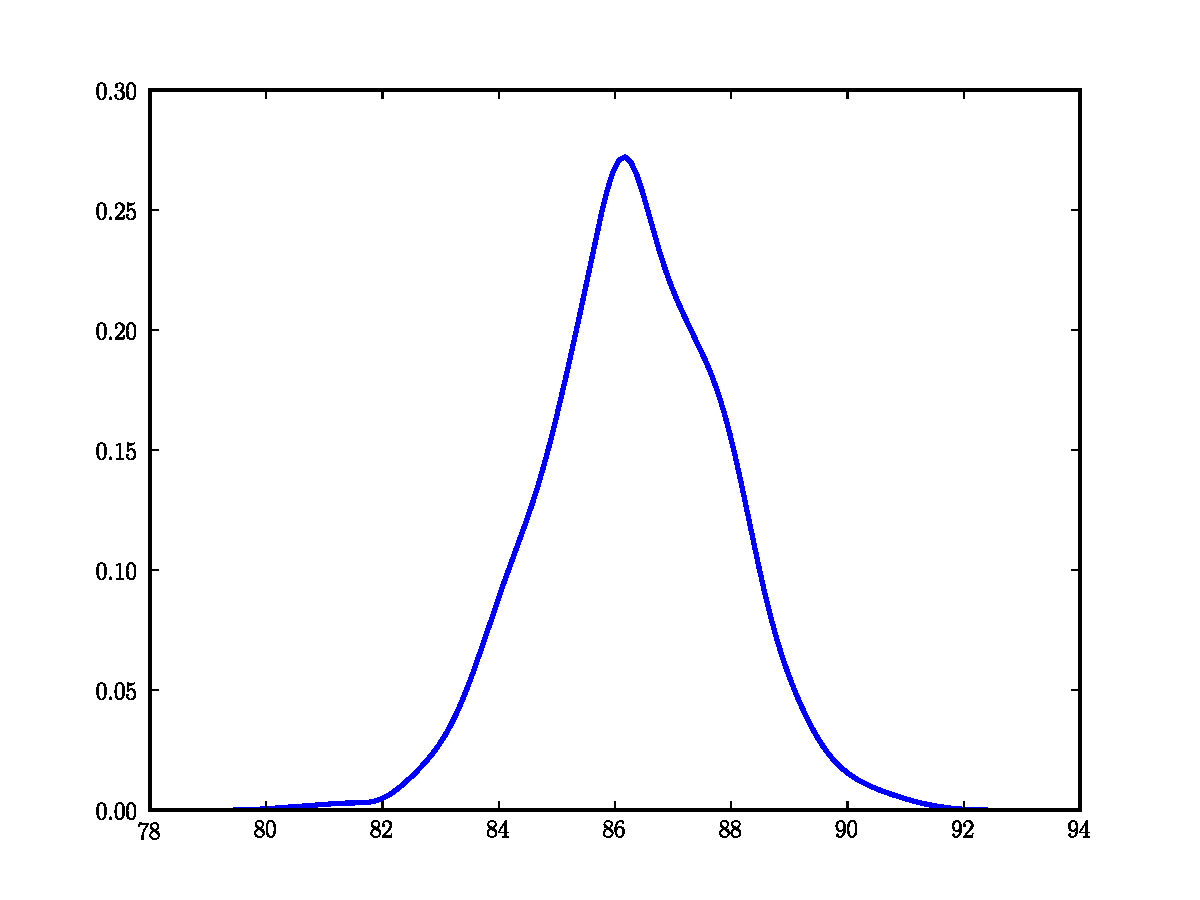
\includegraphics[width=\textwidth]{mu_posterior.pdf}
		\caption{Posterior distribution of $\mu$.}
	\end{subfigure}
	\begin{subfigure}[b]{.49\textwidth}
		\centering
		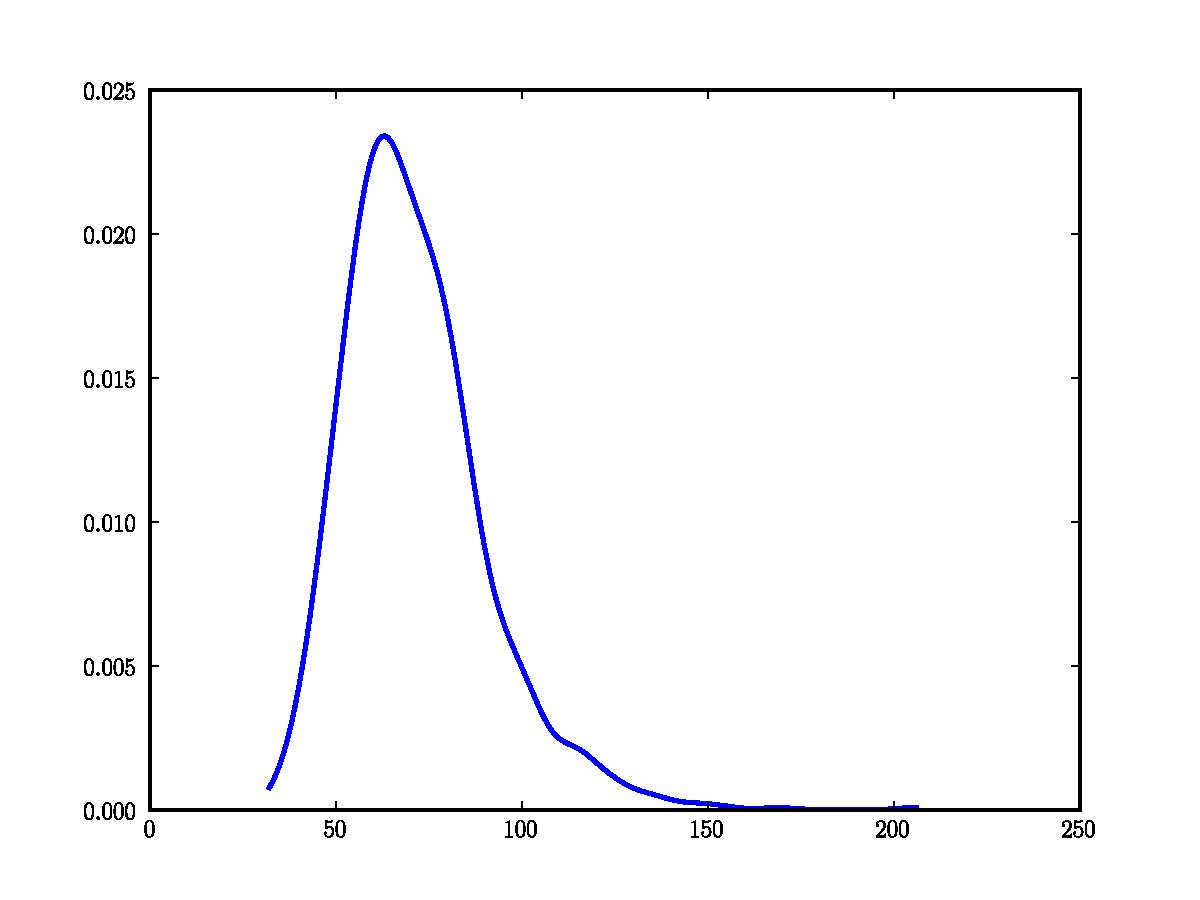
\includegraphics[width=\textwidth]{sigma2_posterior.pdf}
		\caption{Posterior distribution of $\sigma^2$.}
	\end{subfigure}
\end{figure}

\begin{problem}
Plot the kernel density estimators for the posterior distributions of $\mu$ and $\sigma^{2}$.
\end{problem}

Keep in mind that the above plots are of the posterior distributions of the \emph{parameters}, not of the scores. If we would like to compute the posterior distribution of a new score $\tilde{y}$ given our data $\mathbf{y}$ and prior parameters, we compute what is known as the \emph{posterior predictive distribution}: 
\begin{equation*}
\mathbb{P}(\tilde{y} | \mathbf{y}, \lambda) = \int_{\Theta} \mathbb{P}(\tilde{y} | \Theta)\mathbb{P}(\Theta | \mathbf{y}, \lambda) d\Theta
\end{equation*}
where $\Theta$ denotes our parameters (in our case $\mu$ and $\sigma^{2}$) and $\lambda$ denotes our prior parameters (in our case $\mu_{0}, \sigma_{0}^{2}, \alpha,$ and $\beta$).

Rather than actually computing this integral for each possible $\tilde{y}$, we can do this by sampling scores from our parameter samples. In other words, sample 
\begin{equation*}
\tilde{y}_{(t)} \sim N(\mu_{(t)}, \sigma_{(t)}^{2})
\end{equation*}
for each sample pair $\mu_{(t)}, \sigma_{(t)}^{2}$. Now we have essentially drawn samples from our posterior predictive distribution, and we can use a kernel density estimator to plot this distribution from the samples:
\begin{lstlisting}
: n = len(mu_samples)
: score_samples = sp.array([norm.rvs(mu_samples[i], sp.sqrt(sigma2_samples[i])) for i in xrange(n)])
: score_kernel = gaussian_kde(score_samples)
: x_min = min(score_samples) - 1
: x_max = max(score_samples) + 1
: plt.plot(x, score_kernel(x))
: plt.show()
\end{lstlisting}

\begin{figure}[h]
\centering
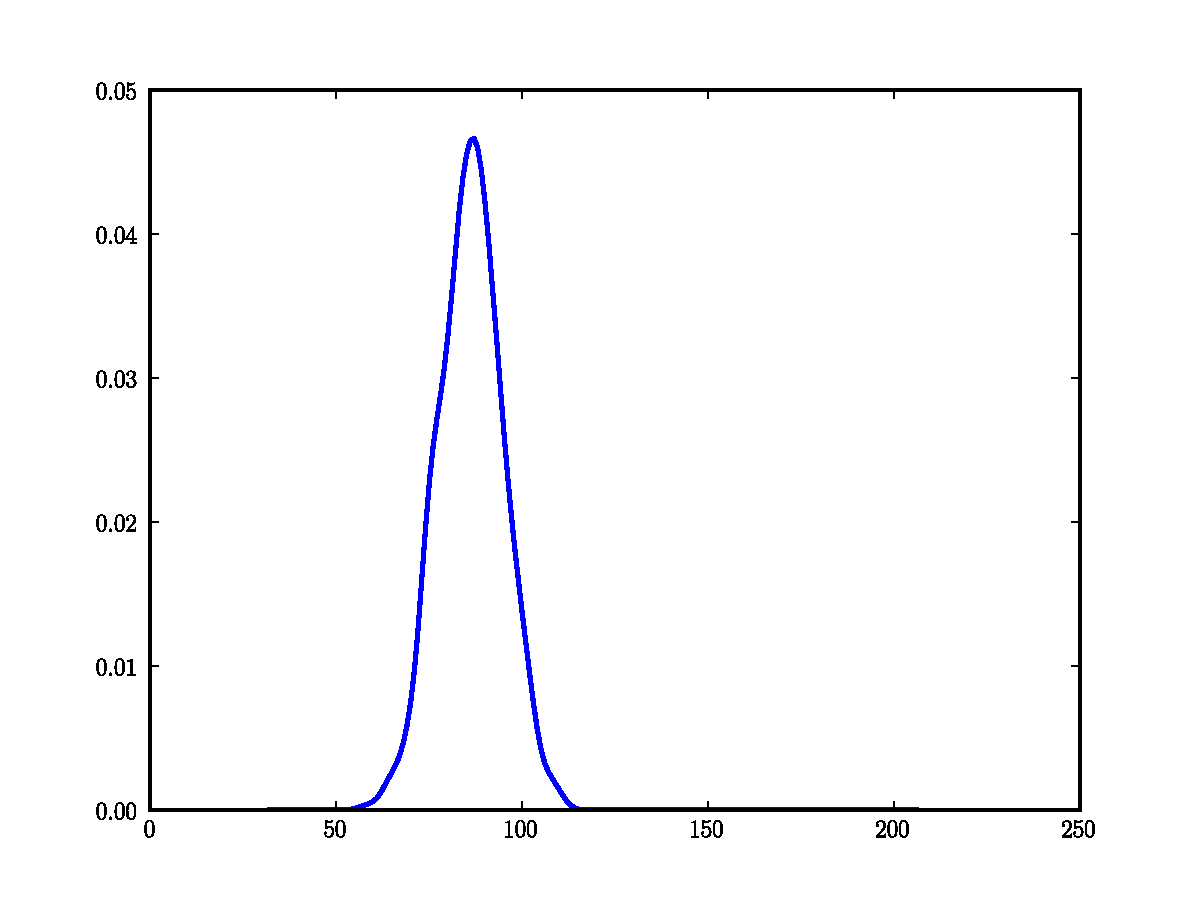
\includegraphics[width=\textwidth]{predictiveposterior.pdf}
\caption{Predictive posterior distribution of exam scores.}
\end{figure}

\begin{problem}
Use your samples to draw samples from the posterior predictive distribution. Plot the kernel density estimator of your sampled scores.
\end{problem}